\begin{question}
\noindent Triangle $P$ has vertices $A(2,3)$, $B(4,3)$ and $C(2,5)$.

\noindent Triangle $P$ is rotated $90^{\circ}$ anticlockwise about the point $(1,1)$ to give triangle $P'$.

\begin{center}
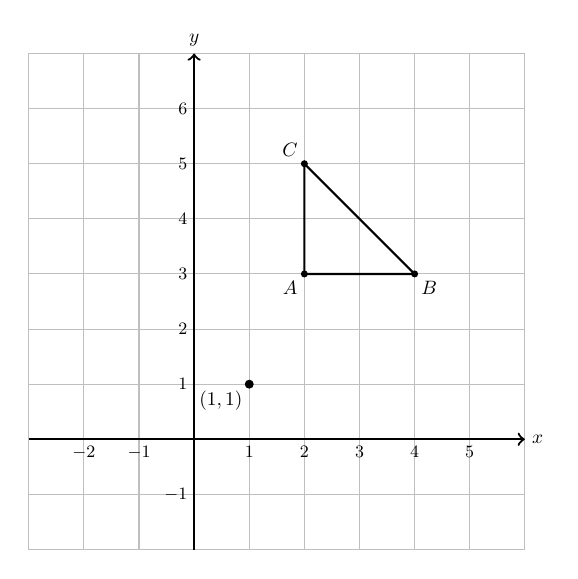
\begin{tikzpicture}[scale=0.7, transform shape]
    % Grid
    \draw[step=1cm, lightgray, thin] (-3,-2) grid (6,7);
    % Axes
    \draw[thick,->] (-3,0) -- (6,0) node[right]{$x$};
    \draw[thick,->] (0,-2) -- (0,7) node[above]{$y$};

    % Axis labels
    \foreach \x in {-2,-1,1,2,3,4,5}
        \node[below] at (\x,0) {\small $\x$};
    \foreach \y in {-1,1,2,3,4,5,6}
        \node[left] at (0,\y) {\small $\y$};

    % Centre of rotation
    \filldraw[black] (1,1) circle (2pt) node[below left]{$(1,1)$};

    % Triangle P
    \draw[thick] (2,3) -- (4,3) -- (2,5) -- cycle;
    \filldraw[black] (2,3) circle (1.5pt) node[below left]{$A$};
    \filldraw[black] (4,3) circle (1.5pt) node[below right]{$B$};
    \filldraw[black] (2,5) circle (1.5pt) node[above left]{$C$};
\end{tikzpicture}
\end{center}

\noindent Draw and label triangle $P'$, the image of triangle $P$ after this rotation.

\vspace{4cm}
\begin{flushright}
    \answerplain{3}
\end{flushright}
\end{question}
